%--------------------------------------------------------------------------
% Introduction
%--------------------------------------------------------------------------

\chapter{Introduction}
\label{cha: introduction}

\section{Background}
\label{sec: intro-background}

Forests are complex, functional systems of interacting and interdependent biological, physical, and chemical components, which creates unique combinations of climate, soil, plant and animal species that result in many different forest types around the world (\cite{blanco_forest_2012}). These ecosystems harbor the vast majority of biological species on Earth (\cite{pan_structure_2013}), account for 80\% of the Earth’s total plant biomass (\cite{kindermann_global_2008}), and store more carbon in biomass and soils than is contained in the atmosphere (\cite{pan_large_2011}). Forests not only play an important role in supporting and maintaining ecological systems and cycles, but also provide a broad range of goods and services to humanity, including social and economic benefits in the long term (\cite{fao_global_2015}). Among the valuable ecosystem goods and services provided by forests are food, fibre, timber, medicine, clean water, aesthetic and spiritual values, climate regulation, a repository of carbon storage, and mitigation of natural hazards such as floods (\cite{pimentel_value_1997}; \cite{pearce_economic_2001}; \cite{blanco_forest_2012}; \cite{pan_structure_2013}; \cite{chazdon_when_2016}).

Nearly 1.6 billion people comprising more than 25\% of the world’s population depend on forest resources for their livelihoods (FAO, 2015a), and another estimated 410 million people are highly dependent on forests for their subsistence and income (Munang et al., 2011). Recent estimates of the global economic values of terrestrial forest ecosystems increased from US\$ 2,769/ha/yr in 1997 to US\$ 5,682/ha/yr in 2011 for tropical forests, and from US\$ 417/ha/yr in 1997 to US\$ 3,137/ha/yr in 2011 for temperate/boreal forests (standardised in terms of 2007 US\$ values; Costanza et al. 2014). The estimates of the economic value of mangrove forests were even higher at US\$ 13,786/ha/yr in 1997 to US\$ 193,843/ha/yr in 2011, which were mainly due to new studies of the value of mangroves in terms of storm protection, erosion prevention, and waste treatment (Costanza et al., 2014).

Despite their renowned importance, however, forests have declined at a staggering rate around the world. Achard et al. (2014) showed that 8.0 M ha/yr of tropical forests were lost between 1990 to 2000, which decreased to 7.6 M ha/yr between 2000 to 2010. Another study by Mayaux et al. (2005) further estimated the annual rates of forest loss in the 1990s for different forest types, particularly 5.8 M ha/yr of humid tropical rainforests, 2.2 M ha/yr of tropical moist deciduous forests, and 0.7 M ha/yr of tropical dry forests. For the period between 2000 to 2012, Hansen et al. (2013) mapped global forest cover change and estimated that a total of 230 M ha of forest were lost due to disturbance while 80 M ha of new forests were established, from which 20 M ha of land experienced both forest loss and forest gain.

Tropical deforestation was mainly driven by agricultural expansion, commercial wood extraction, and infrastructure extension, which were prominently underpinned by economic, political, and institutional factors (Geist \& Lambin, 2002). Agricultural expansion was the main driver of forest cover loss across the tropics between the period of 1980 to 2000, wherein more than 55\% of new agricultural land replaced intact forests and another 28\% came from disturbed forests (Gibbs et al., 2010).

As of 2015, forests occupy 30.6\% of the Earth’s total land area (FAO, 2015b). But although the world's forests decreased from 4.128 B ha in 1990 to 3.999 B ha in 2015 (Keenan et al., 2015), the Food and Agriculture Organisation (FAO) reported that this 25-year period has seen positive results overall, such as in the rate of global net forest loss being cut by over 50\% (i.e., decreased to 0.08\% annually since 2010 being half the rate in the 1990s; Sloan \& Sayer, 2015); the higher attention given to sustainable forest management worldwide (MacDicken et al., 2015); that forests are meeting increasing demand for a variety of forest products and services (Payn et al., 2015); and larger areas being designated for biodiversity conservation (Morales-Hidalgo et al., 2015).

Sustainable forest management is key to ensuring that the ever-increasing demands of a growing human population are met while maintaining ecological functions of healthy forest ecosystems (MacDicken et al., 2015). Forest resources assessment forms an essential part of sustainable forest management, and determining the nature and distribution of land cover is the first step in any forest resources assessment (van der Sanden \& Hoekman, 1999). Gathering better information to monitor and analyse the status and trends on forest resources can further improve forest management (Siry et al., 2005). To this end, accurate estimates of the extent of forests and forest types are indispensable for understanding forest ecosystems and their sustainable use (Foody, 2003), of which remote sensing techniques have been reliably employed over the past several decades as an accurate, systematic, and cost-effective approach for mapping and monitoring forest conditions and changes across a range of scales (Myers, 1988; Franklin, 2001; Dahdouh-Guebas, 2002; Boyd \& Danson, 2005). Combining remote sensing with field observations provides a comprehensive monitoring approach in support of sustainable forest management at a range of scales (Keenan et al., 2015).

\section{Remote sensing of Philippine forests}
\label{sec: intro-rs-phil-forests}

In the Philippines, a nation-archipelago located between the equator and the Tropic of Cancer in Southeast Asia, forests harbor extremely high floral and faunal diversity, and at the same time also serve as home to upland communities that are highly dependent on forest resources (Lasco \& Pulhin, 2000). Studies have cited estimates of the extent of forest cover to be \url{~}90\% of the 30 M ha total land area of the Philippine islands before the Spanish colonisation in 1521, down to \url{~}70\% at the transition of colonial regimes between Spain and America by 1900s, and further reduced to \url{~}60\% during the Japanese occupation of the Philippines from 1942 to 1945 (Kummer, 1992a; Liu et al., 1993; Bankoff, 2007). During the 20th century, the average deforestation rate in the Philippines was estimated to be 148,000 ha/yr (Lasco \& Pulhin, 2000). Recent official forestry statistics in 2015 reported a decline in forest cover from 7.17 M ha in 2003 to 6.84 M ha in 2010 (FMB, 2015). Timber harvesting and agricultural expansion during the Spanish colonisation, followed by rapid and extensive commercial logging in the 20th century were recognised as the main drivers of historical forest loss in the Philippines (Eder, 1990; Kummer, 1992a; Chokkalingam et al., 2006; Bankoff, 2007).\\

\begin{spacing}{1.0}
\begin{longtable}[h!]{ p{1cm} p{5.4cm} p{2.2cm} p{1.9cm} p{2.5cm} }

    \caption[National forest surveys in the Philippines using remotely sensed data.]{National forest surveys in the Philippines using remotely sensed data (adopted from Kummer, 1992b).}
    \label{tab: intro-table1.1}\\
    
    	\toprule
    	Year & Source & Forest & Data & Method of\\ 
		{} & {} & Cover (\%) & Source & Interpretation\\ 
    	\midrule
    	\endhead
    	
		1973 & Lachowski et al. (1979) & 38.0 & Landsat & Digital\\
		1974 & Bruce (1977) & 29.8 & Landsat & Visual\\ 
		1976 & Bonita \& Revilla (1977) & 30.0 & Landsat & Visual\\ 
		1980 & Forestry Development Center (1985) & 25.9 & Landsat & Visual\\
		1987 & Swedish Space Corporation (1988) & 23.7 & SPOT & Visual\\
		2003 & National Mapping \& Resource Information Authority (2004) & No data & Landsat & Visual\\
		2010 & National Mapping \& Resource Information Authority (2014) & No data & Landsat, AVNIR & Visual\\ 
				
    	\bottomrule
    
\end{longtable}

	\noindent Note: At the time of its publication, Kummer's (1992b) study enumerated five national forest surveys using remotely sensed data conducted from the 1970s to the 1980s. Additional surveys conducted from 1990s to the present were included to update this list.\\ \newline
	
\end{spacing}

National forest surveys were conducted in the post-1950s period in support of managing the country's forest resources, which employed either ground-based forest surveys or spaceborne remote sensing technology to produce land and forest cover maps. To date, seven national forest surveys using remotely sensed data have been conducted in the Philippines (Table \ref{tab: intro-table1.1}).

The forest cover maps generated from these past surveys were done mainly by the traditional method of visual or manual interpretation and analysis (except the 1973 maps) using optical remote sensing data, particularly Landsat. While visual interpretation of remotely sensed data is a simple and effective method that can result in excellent spatial information extraction, it is dependent on the extent of knowledge of the analyst regarding the area of study (Bhatta, 2013). Also, since the method depends solely on a human analyst it is more subjective, and tends to be tedious and slow compared to automated digital interpretation techniques (Horning et al., 2010).

The exclusive use of optical satellite data in these mapping surveys meant that cloud cover was a prevalent concern. In particular, tropical regions such as the Philippines feature persistent cloud cover, which affects data availability and temporal consistency of optical data, thereby preventing regular observations (Myers, 1988). The lack of available optical data due to cloud cover contamination may be one of the major limiting factors in the application of the resulting map products from these forest surveys for periodic, consistent, and wall-to-wall national land and forest cover mapping and monitoring (Fig. \ref{fig: intro-fig1.1}).\\

\begin{spacing}{1.0}
\begin{longtable}[h!]{ p{7cm} p{7cm} }

    \caption[Forest cover classification systems used in the 1987, 2003, 2010 maps.]{Forest cover classification systems used in the 1987 and 2003/2010 forest maps.}
    \label{tab: intro-table1.2}\\
    
    	\toprule
    	1987 map & 2003/2010 map\\ 
    	\midrule
    	\endhead
    	
		Closed canopy, mature \textgreater 50\% & Closed forest, broadleaved\\
		Open canopy, mature \textless 50\% & Closed forest, coniferous\\
		Mossy forest & Closed forest, mixed\\
		Pine forest & Open forest, broadleaved\\
		Mangrove forest & Open forest, coniferous\\
		Marshy area and swamp & Open forest, mixed\\
		Submarginal forest & Forest plantation, broadleaved\\ 
		{} & Forest plantation, coniferous\\
		{} & Forest plantation, mangrove (2003 only)\\ 
		{} & Mangrove forest\\ 

    	\bottomrule
    
\end{longtable}	
\end{spacing}

Different forest classification systems were also adopted in these forest surveys. For example, the 2003 and 2010 NAMRIA maps employed similar forest classification schemes based on the FAO Global Forest Resources Assessment (GFRA), but these maps differed from the 1987 Swedish Space Corporation (SSC) map that adopted a different system (Table \ref{tab: intro-table1.2}). The forest definitions used to produce the 1987 map and the 2003/2010 maps were also different from each other (Swedish Space Corporation, 1988; FAO, 2010). These inconsistencies restrict the direct comparison of these maps and render the results incompatible for historical forest cover change analysis.\\

\begin{figure}[!ht] \centering
	\captionsetup[subfigure]{width=2.0in} % <-- Use this to control text which is poorly spaced under a subfigure. 
	\begin{subfigure}[t]{0.32\textwidth}
		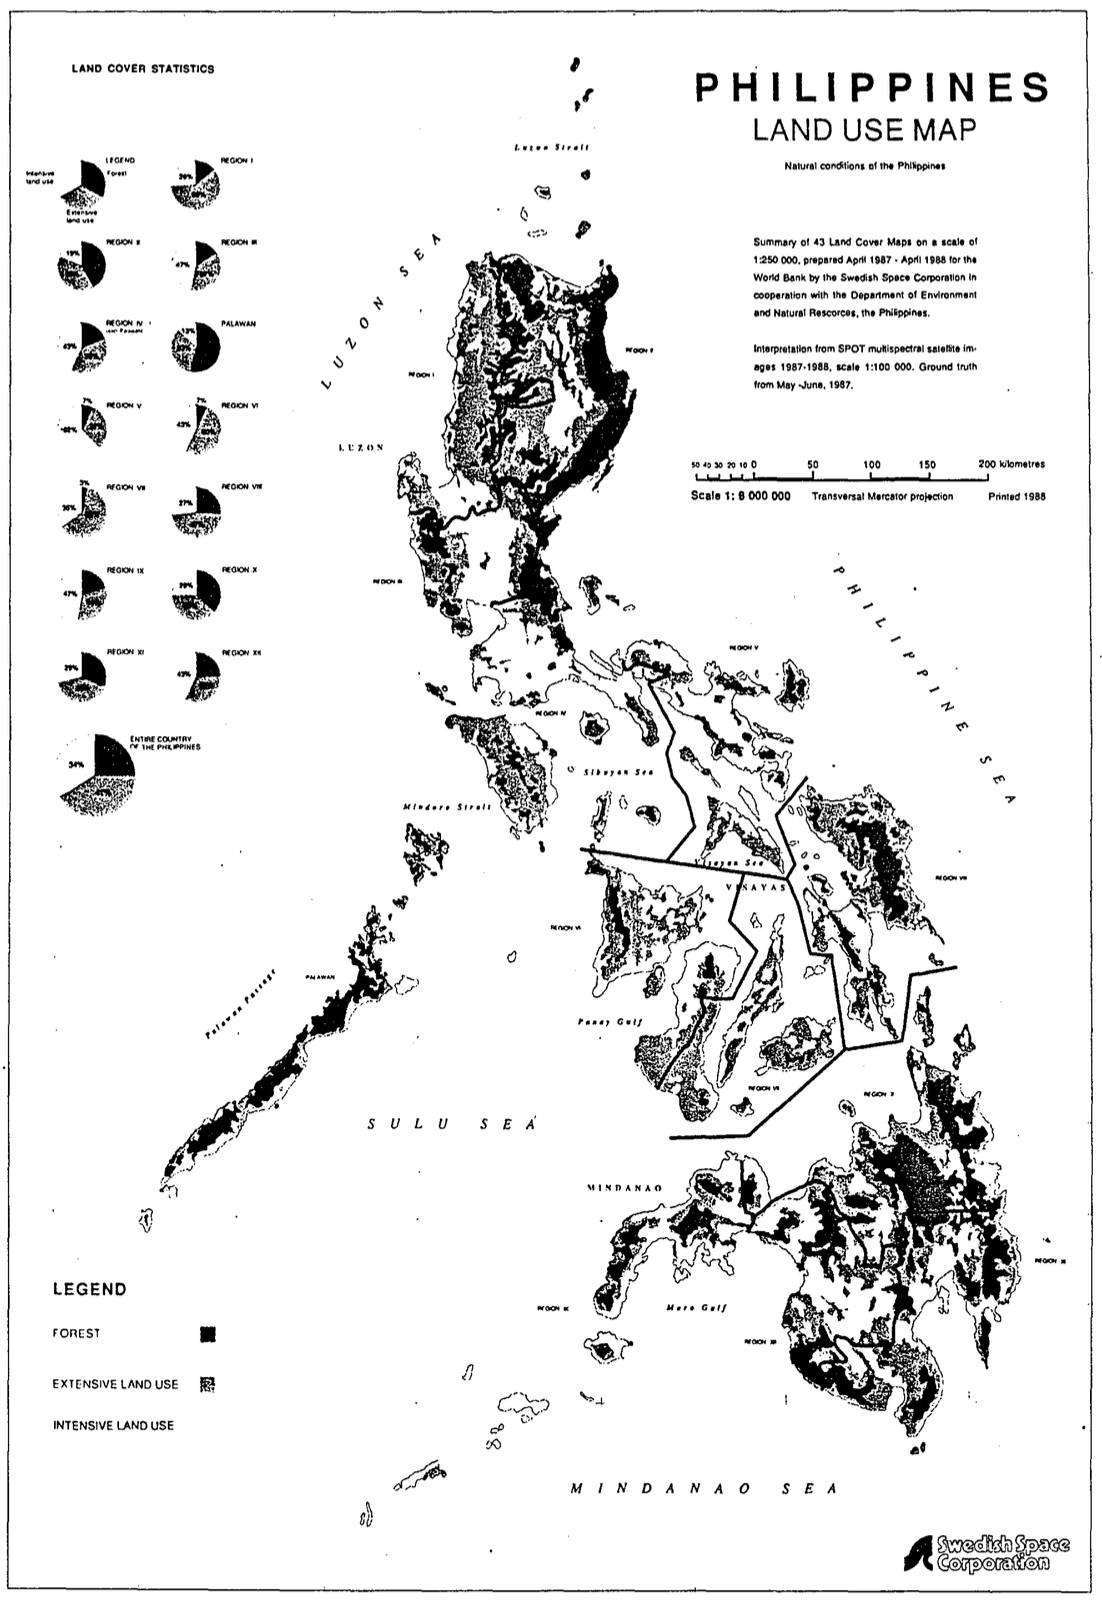
\includegraphics[width=\textwidth]{fig_1987-lc-map.png}
		\caption[SSC/NAMRIA land cover maps.]{}
		\label{fig: intro-fig1.1a}
	\end{subfigure}
	\begin{subfigure}[t]{0.32\textwidth}
		\includegraphics[width=\textwidth]{fig_2003-lc-map.png}
		\caption[SSC/NAMRIA land cover maps.]{}
		\label{fig: intro-fig1.1b}
	\end{subfigure}
	\begin{subfigure}[t]{0.32\textwidth}
		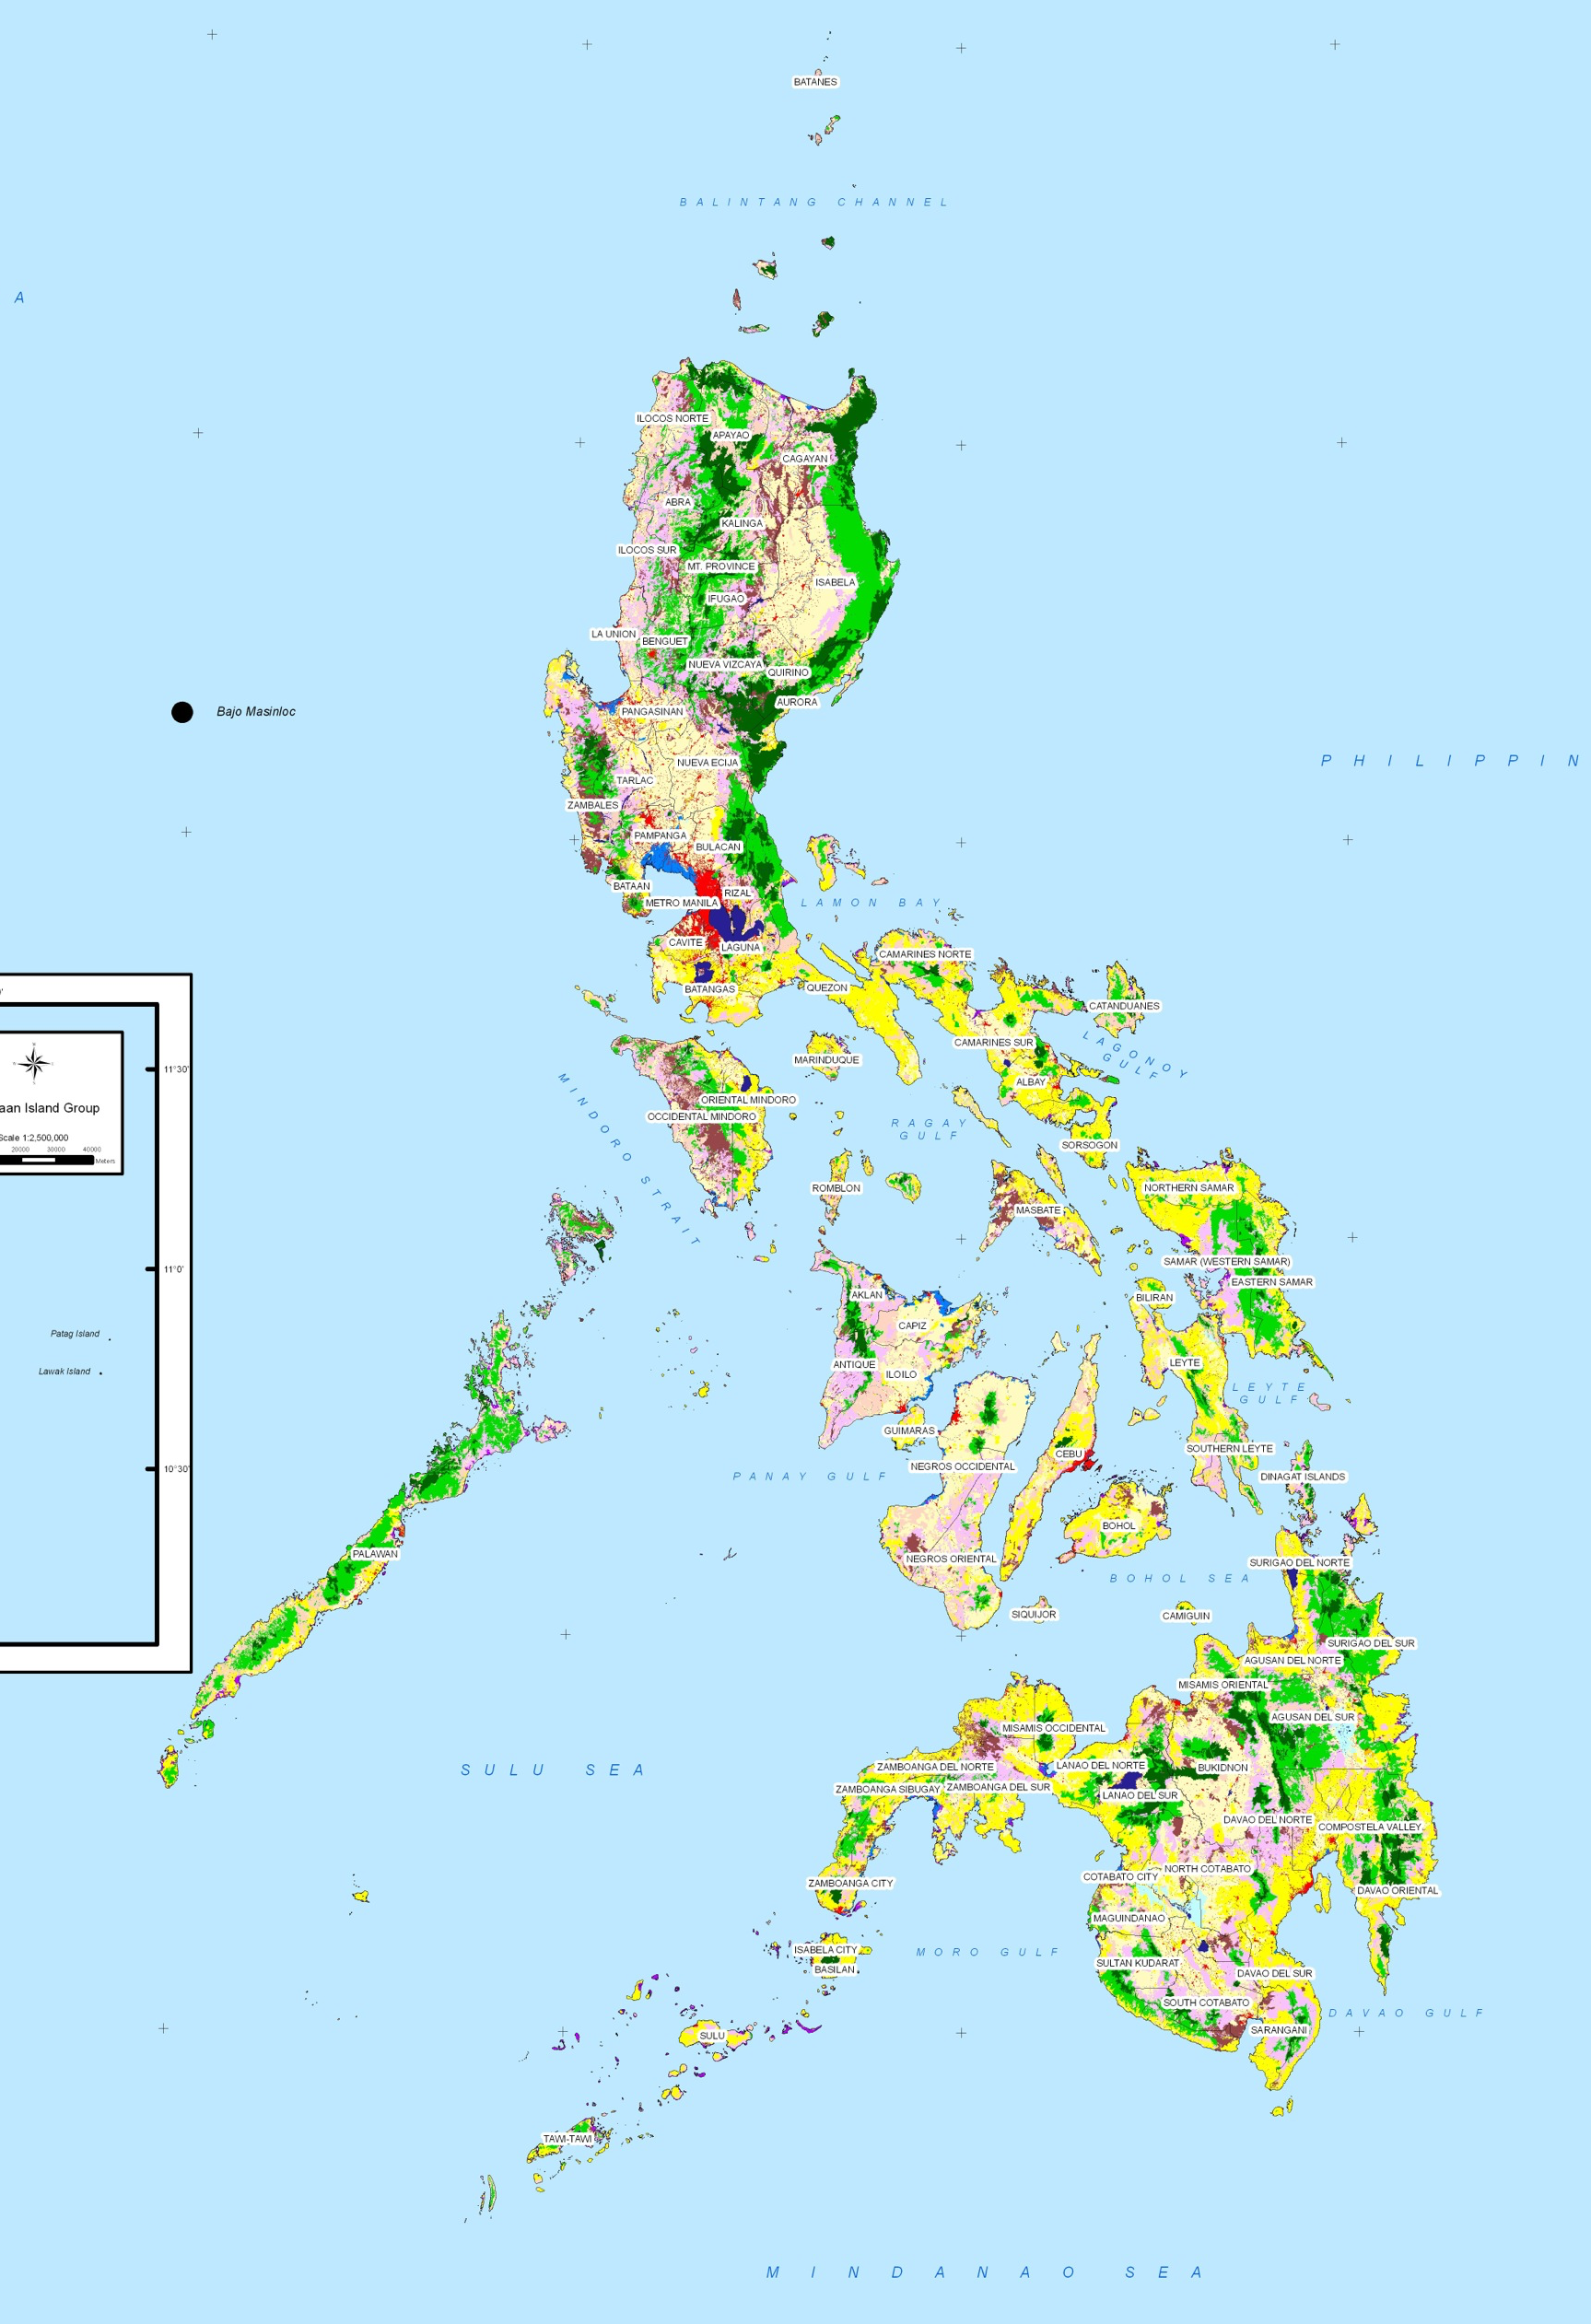
\includegraphics[width=\textwidth]{fig_2010-lc-map.png}
		\caption[SSC/NAMRIA land cover maps.]{}
		\label{fig: intro-fig1.1c}
	\end{subfigure}
	\caption[Recent national land cover maps of the Philippines: (a) 1987 SSC; (b) 2003 NAMRIA; (c) 2010 NAMRIA.]{Recent national land cover maps of the Philippines: (a) 1987 SSC; (b) 2003 NAMRIA; (c) 2010 NAMRIA.}
	\label{fig: intro-fig1.1}
\end{figure}

Finally, there is little known documentation that exists to report on the methods implemented and levels of accuracy achieved in producing many of the forest cover maps from these surveys, except the 1973 and 1987 maps. Lachowski et al. (1979), for the 1973 Landsat-based maps, described the methods undertaken by the mapping work and mentioned an overall accuracy of 85\% to 95\% for the classification of forest types, albeit without sufficient detail. For the 1987 SPOT-based maps, SSC (1988) described their methods and land cover classification system, but did not quantify the accuracy of the results of their interpretation. Kummer (1992b) had cautioned on the reliability of the 1987 SSC map due to major differences with the results of the 1988 Philippine-German Forest Inventory. Reports for other mapping surveys were either not (or no longer) available or were not easily accessible. Since many of these forest mapping surveys employed visual interpretation techniques implemented by expert analysts, the absence of documentation also affects the replicability of the approaches for future work since the knowledge developed from these surveys were ultimately lost.

\section{Overview of the study}
\label{sec: intro-overview-study}

There is an opportunity to explore alternative datasets and methods in support of finding solutions to improve the mapping and monitoring of Philippine forests using remote sensing technology. Synthetic aperture radar (SAR) is an active remote sensing technology that utilises the microwave region of the electromagnetic spectrum that may be used as an alternative (or complement) to optical data for forest mapping and monitoring (discussed in more detail in the next chapter). Innovations in computing technology have leapfrogged over the last two decades and made it possible for computers to handle large remote sensing datasets and to implement sophisticated image processing algorithms for various applications.\\

This research intends to examine the potential of SAR data and digital image processing techniques for mapping forest cover extent and discriminating forest types in the Philippines based on the adopted FAO forest classification system. In contrast to previous national forest mapping surveys using remotely sensed data, which have utilised mainly optical data and visual interpretation for forest cover classification, this study employs image data from an active sensor that can at the onset overcome the limitations brought by persistent cloud cover, and aim to develop a replicable digital image processing and interpretation approach. This study documents the evaluation of the suitability of SAR data for mapping and discriminating forest types by providing quantitative accuracy assessments, and information of the relationships between image data predictor variables and forest types, which are important in developing robust and transparent forest monitoring systems.

This study also adopts the forest categories based on the FAO GFRA for consistency with the recent official national forest cover maps (i.e., 2003 and 2010). One of the key research thrusts in support of planning and decision-making of the National Mapping and Resource Authority (NAMRIA) is to utilise SAR imagery, either as an alternative to or in complementation with optical data, coupled with digital image processing approaches with the aim of developing improved wall-to-wall coverage baseline land and forest cover map products of the entire country on a periodic basis. This study can potentially support NAMRIA’s aims by providing insights on the suitability of radar data and a suite of digital image processing techniques for mapping and monitoring forest extent and forest types in the Philippines.

\section{Thesis structure}
\label{sec: intro-thesis-structure}

This thesis is divided into six chapters. Chapter 1 gives a background of forest ecosystems and remote sensing of forests, and presents an overview of the study. Chapter 2 provides a review of relevant literature on forest applications of synthetic aperture radar, forest classification systems, and the approaches used in this study including cluster analysis, decision trees, texture measures, and object-based image analysis. Chapter 3 describes the study area, the datasets used, and the methods employed. Chapter 4 presents the results of the feature extraction, and clustering and classification procedures. Chapter 5 provides a thorough discussion of the results. Chapter 6 summarizes the study and outlines recommendations for future research and application. The final sections contain the references cited in the text, and the appendices consisting of supplemental figures, rulesets, and scripts used in the study.
